\documentclass[a4paper,twoside]{article}

%% Language and font encodings
\usepackage[spanish]{babel}
\usepackage[utf8]{inputenc}
\usepackage[T1]{fontenc}

%% Sets page size and margins
\usepackage[a4paper,top=3cm,bottom=2cm,left=2.5cm,right=2.5cm,marginparwidth=0.5cm]{geometry}

\usepackage{amsmath}			%Paquete matemático
\usepackage{graphicx}
\usepackage[colorinlistoftodos]{todonotes}

\usepackage{hyperref}		%Paquete empleado para colocar hipervinculos
\hypersetup{
	colorlinks = true,
	linkcolor = black,
}

\usepackage{eurosym}
\usepackage{pdfpages}			%Sirve para incluir PDF en el documento
\usepackage{anysize}			%Podremos colocar imagenes de cualquier tamaño
\usepackage{subfig}				%Nos permitira colocar varias imagenes en una figura
\usepackage{float}				%Podremos crear y colocar boxes donee queramos
\usepackage[export]{adjustbox}

%Colocamos cabeceras y pies de pagina 
%(CONSULTA: http://edicionesoniricas.com/maquetar-latex-encabezados-pies-pagina/)
%(CONSULTA2: https://es.sharelatex.com/learn/Headers_and_footers)
%\bfseries es análogo a \textbf{}
% \leftmark-> Adds name and number of the current top-level structure (section for article) in uppercase letters.
%\rightmark-> Adds name and number of the current next to top-level structure (subsection for article) in uppercase letters.
\usepackage{fancyhdr}		%Paquetes necesarios
\pagestyle{fancy}			%Borra los parametros por defecto
\fancyhf{}
\fancyhead[RO,LE]{\bfseries\thepage}	
\fancyhead[LO,RE]{\bfseries\rightmark}
%Nos aseguramos de que en las paginas plain, no haya ni cabeceras ni lineas
\fancypagestyle{plain}
{
	\fancyhead{} % elimina cabeceras en paginas "plain"
	\renewcommand{\headrulewidth}{0pt} % así como la raya
}

%Definimos las lineas divisoras de las cabeceras y pie de pagina
\renewcommand{\headrulewidth}{1pt}	%Define el grosor de la línea de head
\renewcommand{\footrulewidth}{0pt}		%Define el grosor de la linea foot (Si no queremos linea, 0pt)
\addtolength{\headheight}{0.5pt} % espacio para la raya

%Librerias para introducir código de Matlab
%\usepackage{bigfoot} % to allow verbatim in footnote
\usepackage[numbered,framed]{matlab-prettifier}

\lstset{
	style              = Matlab-editor,
	basicstyle         = \mlttfamily,
	escapechar         = ",
	mlshowsectionrules = true,
}

% Pie de pagina
%\fancyfoot{} % limpia el pie
\fancyfoot[C]{- \thepage -} % número de página centrado

%Nos generará texto para pruebas de maquetado
\usepackage{lipsum}
%---------------------------------------------------------------------------------------------------------------------------------- 
\begin{document}
\begin{titlepage}
	\centering
\Huge{\textbf{CONTROL Y PROGRAMACIÓN DE ROBOTS}} \\
\Huge{\textit{Proyecto de robots manipuladores}}\\

\vspace{1cm}
\LARGE{Grado en Ingeniería Electrónica, Mecatrónica y Robótica}\\
\rule{\textwidth}{0.1mm}
%  %%%%% Este trozo de codigo es para insertar imagenes %%%%%%%
\begin{figure}[h!]
	\centering
	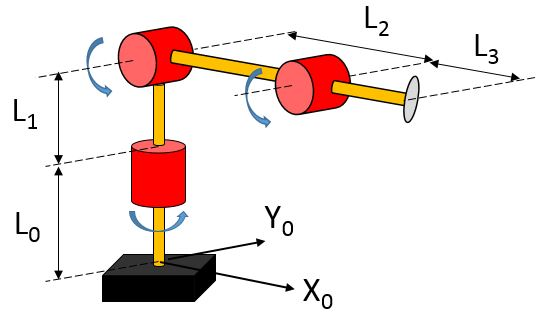
\includegraphics[width=1\textwidth]{brazo_portada}
	%\caption{textodelaleyenda}
\end{figure}
% %%%%%%%%%%%%%%%%%%%%%%%%%%%%%%%%%%%%%%%%%%%%%%%%%%%%%%%%%%%%%
\vspace{3cm}
\rule{\textwidth}{0.1mm}
\Large{\textbf{Autores:} Montes Grova, Marco Antonio\\
 Lozano Romero, Daniel\\
 Mérida Floriano, Javier}
\end{titlepage}
\tableofcontents
\newpage
% %%%%%%%%%%%   INTRODUCCION %%%%%%%%%%%%%%%%%%
\section{Introduccion al proyecto}


% %%%%%%%%%%%%%%%%%%%%%%%%%%%%%%%%%%%%%%%%%%%%%
\section{Análisis Cinemático del brazo}
	\subsection{Modelo Cinemático Directo}
	\subsubsection{Parámetros y estudio del MCD según Denavit-Hartemberg}
	Uno de los modos de estudio del problema cinemático directo de un robot es el procedimiento de Denavit-Hartemberg, el cual se basa en la realización de cambios de sistema de referencia empleando las matrices de transformación homogéneas. Siguiendo una serie de pasos, se llegará a obtener los siguientes parámetros que definen la cinemática directa del robot.\\
	%Tabla de Denavit-Hartenberg
	\begin{center}
		\begin{tabular}{|c||c|c|c|c|}
			\hline
			Articulación & $\theta_{i}$ & $d_{i}$ & $a_{i}$ & $\alpha_{i}$ \\
			\hline
			1 & $\theta_{1}$     				 &   L0+L1    &  			0 			 &  $\frac{\pi}{2}$  \\
			\hline
			2 & $\theta_{2}$ 				 &    0     &L2 & 0  \\
			\hline
			3 & $\theta_{3}$ &    L3    & 			 L2			 &  0\\
			\hline
		\end{tabular}
	\end{center}
	% %%%%%%%%%%%%%%%%%
	% anadir foto del analisis del brazo
	% %%%%%%%%%%%%%%%%%
	
	\subsubsection{Matrices de transformación homogéneas del robot}
	A continuación, se mostrarán las matrices de transformación homogéneas que definen los cambios de sistema de referencia que han hecho posible relacionar el sistema de referencia base con el del efector final. La matriz de transformación homogénea que relaciona un sistema de referencia con el siguiente se define como:\\
	\begin{equation}
	{^{i-1}}A_{i}=Rotz(\theta_{i})*T(0,0,d_{i})*T(d_{i},0,0)*Rotx(\alpha_{i})=
	\begin{pmatrix}
	cos(\theta_{i}) & -sin(\alpha_{i})cos(\theta_{i})	& sin(\alpha_{i})sin(\theta_{i})  & a_{i}cos(\theta_{i})     \\
	sin(\theta_{i}) &  sin(\alpha_{i})cos(\theta_{i})	& -sin(\alpha_{i})cos(\theta_{i}) & a_{i}sin(\theta_{i})     \\
	0 		&  			sin(\alpha_{i})   		& 		cos(\alpha_{i})			  & d_{i}\\
	0 		&					0				&				0  		  		  & 1
	\end{pmatrix}
	\end{equation}
	
	Ahora que se ha definido la matriz general, se definirán las matrices de transformación homogéneas de cada cambio de sistema de referencia del robot: \\
	
	\[ {^0}A_{1} =
	\left( \begin{array}{cccc}
	cos(\theta_{1}) &  0 &  sin(\theta_{1}) & 0  \\ 
	sin(\theta_{1}) &  0 & -cos(\theta_{1}) & 0  \\
	0		&  1 &		 0 			& L0+L1 \\
	0		&  0 & 		 0			& 1
	\end{array} \right) \]
	
	\[ {^1}A_{2} =
	\left( \begin{array}{cccc}
	cos(\theta_{2}) & -sin(\theta_{2}) & 0 & L2cos(\theta_{2}) \\ 
	sin(\theta_{2}) & cos(\theta_{2})  & 0 & L2sin(\theta_{2})  \\
	0 		 	   & 			0 			& 1	& 		0 			 \\
	0		 	   &			 0			& 0	& 		1
	\end{array} \right) \]
	
	\[ {^2}A_{3} =
	\left( \begin{array}{cccc}
	cos(\theta_{3}) &  -sin(\theta_{3}) &  0 & L3cos(\theta_{3})   \\ 
	sin(\theta_{3}) &  cos(\theta_{3}) &  0 & L3sin(\theta_{3})   \\
	0 					 &  0 &  				1 					  & 0 \\
	0 					 &  0 & 				 0					  & 1
	\end{array} \right) \]
	
	\subsubsection{Ecuaciones simbólicas del MCD}
	A partir de estos parámetros será posible obtener las matrices de transformación homogéneas asociadas a cada traslación y giro de sistema de referencia. Si se premultiplican las matrices desde la base hasta el punto final del brazo (efector final), la matriz de transformación obtenida será:
	\begin{equation}
	{^3}T_{0} = 
	\left( \begin{array}{cccc}
	cos(\theta_{2}+\theta_{3})cos(\theta_{1})  & -sin(\theta_{2}+\theta_{3})cos(\theta_{1}) &  -sin(\theta_{1})  & cos(\theta_{1})[L3cos(\theta_{2}+\theta_{3}) + L2cos(\theta_{2})] \\ 
	cos(\theta_{2}+\theta_{3})sin(\theta_{1})  & -sin(\theta_{2}+\theta_{3})sin(\theta_{1}) & cos(\theta_{1})  & sin(\theta_{1})[L3cos(\theta_{2}+\theta_{3}) + L2cos(\theta_{2})] \\
	sin(\theta_{2}+\theta_{3})		 		  &		 cos(\theta_{2}+\theta_{3})		        & 		0 			& L0 + L1 + L3sin(\theta_{2}+\theta_{3}) + L2sin(\theta_{2})	 \\
	0						  &		 	0  									&       0		    &   1
	\end{array} \right)
	\end{equation}
	Donde se puede extraer que la matriz de orientación del efector final y la posición del mismo respecto al sistema de referencia de la base son:
	\[ noa =
	\left( \begin{array}{ccc}
cos(\theta_{2}+\theta_{3})cos(\theta_{1})  & -sin(\theta_{2}+\theta_{3})cos(\theta_{1}) & -sin(\theta_{1})  \\ 
cos(\theta_{2}+\theta_{3})sin(\theta_{1})  & -sin(\theta_{2}+\theta_{3})sin(\theta_{1}) & cos(\theta_{1})  \\
sin(\theta_{2}+\theta_{3})		 		  &		 cos(\theta_{2}+\theta_{3})		        & 		0 						 			 
	\end{array} \right) \]
	
	\[ p =
	\left( \begin{array}{c}
	cos(\theta_{1})[L3cos(\theta_{2}+\theta_{3}) + L2cos(\theta_{2})] \\ 
	sin(\theta_{1})[L3cos(\theta_{2}+\theta_{3}) + L2cos(\theta_{2})] \\ 
	L0 + L1 + L3sin(\theta_{2}+\theta_{3}) + L2sin(\theta_{2})			 
	\end{array} \right) \]
	
	\subsection{Modelo Cinemático Inverso}
	
	En lo que a la resolución del modelo cinemático inverso del robot respecta, se basará en obtener los valores de las variables articulares a partir de la posición del efector final. Por tanto, se partirá de las ecuaciones del vector $p$:
	
	\begin{center}
		$px=cos(\theta_{1})[L3cos(\theta_{2}+\theta_{3}) + L2cos(\theta_{2})]$ \\ 
		$py=sin(\theta_{1})[L3cos(\theta_{2}+\theta_{3}) + L2cos(\theta_{2})]$ \\ 
		$pz=L0 + L1 + L3sin(\theta_{2}+\theta_{3}) + L2sin(\theta_{2})$			
	\end{center}
	
	Para obtener las ecuaciones que definen el valor de $\theta_{1}$,$\theta_{2}$ y $\theta_{3}$, se trabajará con las funciones que definen px,py y pz. Será necesario definir los ángulos empleando la función atan2 de \textit{Matlab}, ya que de ese modo se distinguirá en qué cuadrante se encuentra la tangente.\\
	Por tanto el objetivo es obtener el valor del seno y el coseno de cada ángulo.\\
	
	Se comenzará obteniendo el valor de $\theta_{1}$. Para ello se define:\\
	\begin{center}
		$ A = \sqrt{px^{2}+py^{2}} = L3cos(\theta_{2}+\theta_{3}) + L2cos(\theta_{2})$
	\end{center}
	de ese modo, se obtiene $\theta_{1}$ como:\\
	\begin{equation}
	\theta_{1}=atan2(sin(\theta_{1}),cos(\theta_{1}))=atan2(\frac{py}{A},\frac{px}{A})
	\end{equation}
	Para obtener el valor de $\theta_{3}$, se comenzará a partir de pz y, se definirá la siguiente variable auxiliar:\\
	\begin{center}
		$ B=pz-L1-L0=L3sin(\theta_{2}+\theta_{3}) + L2sin(\theta_{2})$
	\end{center}
	Si se trabaja con las dos variables auxiliares creadas, A y B, y se crea la nueva variable C, se conseguirá obtener el valor del ángulo deseado:\\
	\begin{center}
		$C= A^{2} + B^{2} = L2^{2}+ 2L2L3cos(\theta_{3}) + L3^{2} $
	\end{center}
	
	Cómo último paso para obtener el valor de $\theta_{3}$, se despejará el valor del coseno del mismo:\\
	\begin{center}
		$ (cos(\theta_{3})) = \frac{C-L2^{2}-L3^{2}}{2L2L3} $
	\end{center}
	Por tanto, $\theta_{3}$ se define como:\\
	\begin{equation}
	\theta_{3}=\beta -atan2(sin(\theta_{3}),cos(\theta_{3}))=\beta-atan2(\pm \sqrt{1-(\frac{C-L2^{2}-L3^{2}}{2L2L3})^{2}},\frac{C-L2^{2}-L3^{2}}{2L2L3} )
	\end{equation}
	
	\newpage
	Por último, se hallará el valor de la variable articular $\theta_{2}$. Para ello, se partirá de la ecuación A y se desarrollará empleando la fórmula del coseno del ángulo doble. La ecuación quedará de la forma: \\
	\begin{center}
		$A=L3cos(\theta_{2}+\theta_{3})+L2cos(\theta_{2})=L3[cos(\theta_{2})cos(\theta_{3})-sin(\theta_{2})sin(\theta_{3})]+L2cos(\theta_{2})=$\\ \vspace{0.3cm} $L3cos(\theta_{2})cos(\theta_{3})-L3sin(\theta_{2})sin(\theta_{3})+L2cos(\theta_{2})$
	\end{center}
donde será de ayuda despejar la función A en una suma de un término por el seno de $ \theta_{2}$ y otro término por el coseno del mismo ángulo. De ese modo será posible intentar obtener dicho ángulo empleando un cambio a coordenadas polares:
	\begin{center}
		$A=cos(\theta_{2})[L3cos(\theta_{3})+L2]-sin(\theta_{2})[L3sin(\theta_{3})]$\\
		\vspace{0.3cm}
		\fbox{%
			\begin{minipage}[b][1.2cm][c]{0.9\textwidth}
				$\rho cos(\alpha)=L3cos(\theta_{3})+L2$ \hspace*{3cm} $\rho=\sqrt{(L3sin(\theta_{3}))^{2}+(L3cos(\theta_{3})+L2)^{2}} $\\
				$\rho sin(\alpha)=L3sin(\theta_{3})$ \hspace*{3.8cm} $\alpha=atan2(L3sin(\theta_{3}),L3cos(\theta_{3})+L2)$\\
			\end{minipage}
		}\hfill
	\end{center}
	Sustituyendo en la ecuación A y empleando la fórmula del coseno del ángulo suma, se podría definir:\\
	\begin{center}
	$A=\rho cos(\theta_{2})cos(\alpha)-\rho sin(\theta_{2})sin(\alpha)$ $\rightarrow$ $A=\rho cos(\theta_{2}+\alpha)$
	\end{center}
	
	Despejando el valor del coseno $\theta_{3}$ se obtendrá:
	\begin{equation}
	\theta_{2}=atan2(\pm \sqrt{1-(\frac{A}{\rho})^{2}},\frac{A}{\rho})-\alpha
	\end{equation}
	De ese modo, la solución del problema cinemático inverso está formada por siguientes ecuaciones:
	\begin{center}
		$\theta_{1}=atan2(sin(\theta_{1}),cos(\theta_{1}))=atan2(\frac{py}{A},\frac{px}{A})$ \\
		$\theta_{2}=atan2(\pm \sqrt{1-(\frac{A}{\rho})^{2}},\frac{A}{\rho})-\alpha$ \\
		$\theta_{3}=\beta -atan2(sin(\theta_{3}),cos(\theta_{3}))=\beta-atan2(\pm \sqrt{1-(\frac{C-L2^{2}-L3^{2}}{2L2L3})^{2}},\frac{C-L2^{2}-L3^{2}}{2L2L3} )$
	\end{center}
	\subsection{Jacobiano del robot y análisis de puntos singulares}
	
	\newpage
\section{Análisis Dinámico del brazo}
Una vez analizada la cinemática del brazo, se debe pasar a realizar un análisis dinámico del mismo. Este análisis nos muestra la relación que existe entre las intensidades aplicadas a los motores delas articulaciones del robot y las posiciones, velocidades y aceleraciones de dichas articulaciones.\\

La ecuación que permite obtener dicha relación es la siguiente:\\

	\begin{equation}
	K_tRI_m=(M(q)+J_mR^2)qdd+(C(q,qd)+B_mR^2)qd+G(q)+F(qd)
	\end{equation}\\
	
En la ecuación anterior, se tiene, en el término de la izquierda, las matrices de constantes de par de cada motor ($K_t$) y de reductoras ($R$) e intensidades ($I_m$) aplicadas a cada motor.\\

Por otro lado, en el término de la derecha encontramos las matrices de inercia de los eslabones ($M(q)$) y de los motores ($J_m$), la matriz de términos de Coriolis ($C(q,qd)$) y la de términos viscosos de los motores ($B_m$), y las matrices de términos gravitatorios ($G(q)$) y de fricciones ($F(qd)$), donde esta última no se tendrá en cuenta para la estimación del modelo.\\

Aparecen también los vectores columna $q$, $qd$ y $qdd$ que corresponden, respectivamente, a los valores de posición, velocidad y aceleración de las articulaciones.\\

Para tratar de hallar la ecuación anterior, se va a realizar un método recursivo que se basa en la segunda ley de Newton denominado algoritmo de Newton-Euler, el cual obtiene los esfuerzos/pares aplicados en cada articulación. Dicho algoritmo ha sido proporcionado en clase por lo que no se explicará aquí. Sí decir que como del robot sólo se conocen las longitudes de los eslabones y algunos parámetros dinámicos (reductoras y constantes de par) se realizará el cálculo con variables simbólicas que serán estimadas y sustituidas más adelante.\\

El resultado que se desea obtener con dicho algoritmo es el siguiente:\\
\begin{equation}
T=M(q)qdd+V(q,qd)+G(q),
\end{equation}
donde el término $V(q,qd)$ hace referencia al conjunto $C(q,qd)qd$.\\

Como el algoritmo anterior obtiene el resultado total, se debe derivar el mismo para poder hallar las matrices aisladas. Por ello, el resultado $T$ se deriva respecto a $qdd$ para obtener la matriz $M(q)$. Acto seguido restar la matriz obtenida multiplicada por $qdd$ al valor de $T$ para eliminarlo y obtener las otras dos matrices.\\

El siguiente paso consiste en derivar la nueva $T$ respecto a la constante de gravedad $g$, puesto que aparece únicamente en los términos gravitatorios. Así, y multiplicando por $g$ a posteriori, se obtiene la matriz $G(q)$. Para hallar la matriz $V(q,qd)$ basta con restar a la $T$ resultante de extraer la matriz de inercia la $G(q)$ anterior.\\

Una de las características que hay que tener en cuenta del algoritmo de Newton-Euler es que no tiene en cuenta las viscosidades e inercias de los motores, por lo que hay que añadirlas a posteriori obteniendo las matrices $Ma(q)=M(q)+J_mR^2$ y $Va(q,qd)=V(q,qd)+B_mR^2qd$.\\

Una vez realizado todo esto se ha obtenido el modelo dinámico simbólico del robot, que se va a suponer correcto pues únicamente consiste en seguir unos pasos descritos en clase, pero que, si se desease, se podría comparar con un robot diseñado en Robotics Toolbox de Matlab asignando valores a los parámetros y realizando un mismo experimento para ambos modelos, tomando como referencia correcta el último de ellos.\\




	

\section{Obtencion de los parametros dinamicos del robot}
Debido a que no se conocen los parametros dinamicos del robot, sera posible estimarlos mediante una serie de experimentos y aproximaciones. Se ha optado por aplicar el algoritmo de Newton-Euler, el cual es un procedimiento recursivo que se basa en la segunda ley de Newton. Este algoritmo nos dara los esfuerzos en las articulaciones.\\
Por tanto, trabajando con Matlab, si se definen todas esas variables del robot de manera simbolica y se corre el algoritmo, se obtendran los pares que sufren las articulaciones.\\
Las variables que se busca estimar del robot seran las siguientes:
\begin{center}
		$ I_{11} =
	\begin{bmatrix}
	I_{11xx} & I_{11xy} & I_{11xz}\\ 
	I_{11yx} & I_{11yy} & I_{11zz}\\ 
	I_{11zx} & I_{11zy} & I_{11zz}
	\end{bmatrix}$

	$ I_{22} =
	\begin{bmatrix}
	I_{22xx} & I_{22xy} & I_{22xz}\\ 
	I_{22yx} & I_{22yy} & I_{22zz}\\ 
	I_{22zx} & I_{22zy} & I_{22zz}
	\end{bmatrix}$
TERMINAR DE METER MATRICES LOCO
\end{center}
\begin{itemize}
	\item HABLAR UN POCO DE LA NECESIDAD DE ESTIMAR LOS PARAMETROS DE NEWTON EULER
	\item HABLAR DE COMO SE OBTUVO GAMMA SIM Y TETHA SIM
	\item HABLAR DE LA SIMPLIFICACION A PARAMETROS LI
	\item HABLAR DE LOS EXPERIMENTOS DE LOS SENOS
	\item HABLAR DE LA OPTIMIZACION Y ESTIMACION DE LOS PARAMETROS
	\item CONTRUCCION DEL MODELO A PARTIR DE LOS PARAMETROS
	\item COMPARATIVA ROBOT REAL Y MODELOS. CONCLUSIONES
\end{itemize}
	\subsection{Obtencion del modelo para estimar los parametros}
	\subsection{Estimacion de parametros dinamicos}
	\subsection{Calculos estadisticos}
	\subsection{Analisis de resultados}
\section{Control Cinematico del robot}
\begin{itemize}
	\item HABLAR SOBRE QUE ES EL CONTROL CINEMATICO Y LAS MOVIDAS DE LOS GENERADORES DE TRAYECTORIAS
	\item TIPOS DE TRAYECTORIAS. COMO LA GENERAMOS
	\item INTERPOLADORES DE TRAYECTORIAS
	\item IMPLEMENTACION, GRAFICAS Y CONCLUSCIONES 
\end{itemize}
	\subsection{Generador de trayectorias punto a punto}
	\subsection{Generador de trayectorias lineal}
	\subsection{Pruebas y conclusiones}
\section{Control Dinámico del brazo}
En esta última parte del proyecto, una vez se conoce el modelo del robot en las diferentes configuraciones, se pasará a buscar implementar un control dinámico sobre el mismo.Para poder implementar controladores sobre nuestro robot, será necesario obtener una función de transferencia matemática a modo de modelo que se asemeje al robot real.\\
Una vez se tenga un modelo lineal de cada articulación del robot, junto con el generador de trayectorias creado anteriormente, se buscará que el robot siga una trayectoria predefinida.\\

	\subsection{Obtención del modelo lineal de las articulaciones del brazo}
Para obtener la función de transferencia de cada articulación del robot, se linealizará la ecuación dinamica que define cada motor en un punto de equilibrio en torno a velocidades nulas. Por lo tanto, las consideraciones que se tendrán en cuenta para linealizar la ecuación dinamica que define el comportamiento de cada articulacion del robot son:
\begin{itemize}
	\item Velocidades de equilibrio
	\begin{center}
		$ \dot{q_{eq}}=0 rad/s $\\
		$ \dot{q} =\dot{q_{eq}}+\Delta\dot{q}$
	\end{center}
	\item Aceleraciones de equilibrio
\begin{center}
	$ \ddot{q_{eq}}=0 rad/s $\\
	$  $
	$ \ddot{q} =\ddot{q_{eq}}+\Delta\ddot{q}$
\end{center}
\end{itemize}

Ademas de ello, se aplicarán una serie de simplificaciones a la ecuación dinámica. A continuación, se mostrarán las ecuaciones dinámicas de los motores:\\
\begin{center}
	$$
	\begin{pmatrix}
	 \tau_{1} \\
	 \tau_{2} \\
	 \tau_ {3}
	\end{pmatrix}=
	\begin{pmatrix}
	Kt_{1}R_{1}Im_{1}  \\
	Kt_{2}R_{2}Im_{2}  \\
	Kt_{3}R_{3}Im_{3}
	\end{pmatrix} =
	\begin{pmatrix}
	Ma_{11} & Ma_{12} & Ma_{13}  \\
	Ma_{21} & Ma_{22} & Ma_{23}  \\
	Ma_{31} & Ma_{32} & Ma_{33}
	\end{pmatrix}
	\ddot{q}+
	\begin{pmatrix}
	Va_{1} \\
	Va_{2} \\
	Va_{3} \\
	\end{pmatrix}
	\dot{q}+
	\begin{pmatrix}
	Ga_{1}  \\
	Ga_{2}  \\
	Ga_{3}\\
	\end{pmatrix}
	$$
\end{center}
donde se asume que dentro de los términos de inercia y de Coirolis se han tenido en cuenta las inercias y fricciones viscosas de los motores.\\

La primera simplificación del modelo que se hará para poder linealizar el modelo en torno a un punto de operación, será suponer la matriz de inercias diagonal y, además de ello, se cogerá el valor medio de todos los senos y cosenos de tal modo que únicamente se tomen los valores de inercias medios. De éste modo, se desacoplará el sistema.\\
En cuando a la matriz de términos de Coirolis, únicamente aportarán a la linealización la fricción viscosa de los motores. Por último, la gravedad se despreciará para obtener un modelo, de tal modo que, se emplearán las siguientes ecuaciones para obtener los modelos de las articulaciones del robot:
\begin{equation}
	\begin{pmatrix}
	Kt_{1}R_{1}Im_{1}  \\
	Kt_{2}R_{2}Im_{2}  \\
	Kt_{3}R_{3}Im_{3}
	\end{pmatrix} =
	\begin{pmatrix}
	Ma_{11} & 0 	  & 0  \\
		0   & Ma_{22} & 0  \\
		0   & 0   	  & Ma_{33}
	\end{pmatrix}
	\ddot{q}+
	\begin{pmatrix}
	Va_{1} \\
	Va_{2} \\
	Va_{3} \\
	\end{pmatrix}
	\dot{q}
\end{equation}

A continuación, se obtendrá el modelo de la primera articulación y, el procedimiento será análogo para las restantes:
\begin{center}
	$Kt_{1}R_{1}Im_{1}(t)=Ma_{11}\ddot{q_{1}(t)} + Va_{1}\dot{q_{1}(t)}$
\end{center}
Se realizará una transformación al dominio de Laplace y, posteriormente, se expresará en forma de función de transferencia:
\begin{center}
	$Kt_{1}R_{1}Im_{1}(s)=s^{2}Ma_{11}q_{1}(s) + sVa_{1}q_{1}(s)$ $\rightarrow$ $\frac{q_{1}(s)}{Im_{1}(s)}=\frac{Kt_{1}R_{1}}{s(Ma_{11}s+Va_{1})}$
\end{center}

Por lo tanto, se definirá el modelo de cada articulación cómo:
\begin{equation}
	G_{1}(s)=\frac{Kt_{1}R_{1}}{s(Ma_{11}s+Va_{1})} \hspace{1cm} G_{2}(s)=\frac{Kt_{2}R_{2}}{s(Ma_{2}s+Va_{2})} \hspace{1cm} G_{3}(s)=\frac{Kt_{3}R_{3}}{s(Ma_{33}s+Va_{3})}
\end{equation}

	\subsection{Diseño de controladores}
	En éste apartado, se analizará cómo se hayarán los controladores que, posteriormente se implementarán sobre el robot para hacer que se traslade a lo largo de una trayectoria que se generará mediante el control cinemático.\\
	A continuación se hará un análisis teórico de cada controlador y del calculo de los mismos.
	\subsubsection{Controlador PD/PID}
	\subsubsection{Controlador PD/PID con compensación de gravedad}
	Para implementar éste controlador, se parte de la base de que, aunque la gravedad es una perturbación mantenida, se puede
modelar, ya que se conoce de la obtención del modelo dinámico los efectos de la gravedad en el modelo del robot.\\
Por tanto, para implementar un controlador con compensación de gravedad se le sumará a la señal de control generada por el
controlador los efectos de la gravedad en el robot.\\
Este bloque que añade los efectos de la gravedad tendrá como entrada la posición actual del robot y la salida será la compensación de la señal de control. El esquema de montaje de éste tipo de control se muestra a continuación:
%\begin{figure}[h!]
%	\centering
%	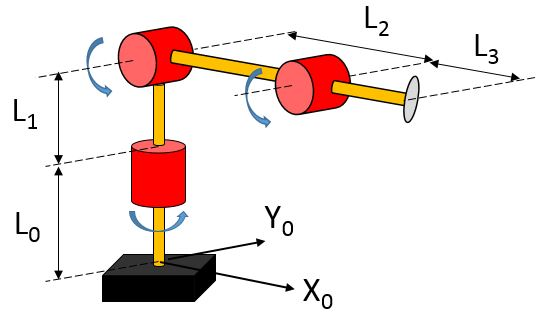
\includegraphics[width=1\textwidth]{brazo_portada}
%	\caption{textodelaleyenda}
%\end{figure}
	\subsubsection{Controlador PD/PID con compensación de dinámica (Feedforward)}
	Para implementar éste controlador, también conocido como \textit{Feedforward}, se modificará el modelo del robot de tal modo que se le añada a la ecuación dinámica un nuevo parámetro:
	\begin{equation}
		I_{i}m= M_{A}(q)\ddot{q_{ref}} + C(q,\dot{q})\dot{q} + G_{A}(q) + u
	\end{equation}
	si con el control anterior se compensaban los terminos gravitatorios del modelo del robot, en éste caso, también se
	compensarán los términos de Coirolis del modelo, los cuales fueron despreciados al obtener el modelo a partir del cuál se
	diseño el controlador.
	\subsubsection{Controlador PD/PID con par calculado}
	\subsection{Analisis de controladores}

\section{Anexos}
	\subsection{Conclusiones (A LO MEJON SI A LO MEJON NO)}
	\subsection{Codigos de programacion}
	\subsection{Montajes en Simulink}

\end{document}